% C-SE Block Architecture Diagram (standalone TikZ)
\documentclass[tikz,border=3pt]{standalone}
\usepackage{tikz}
\usetikzlibrary{shapes.geometric, arrows.meta, positioning, calc, backgrounds, fit}

\begin{document}
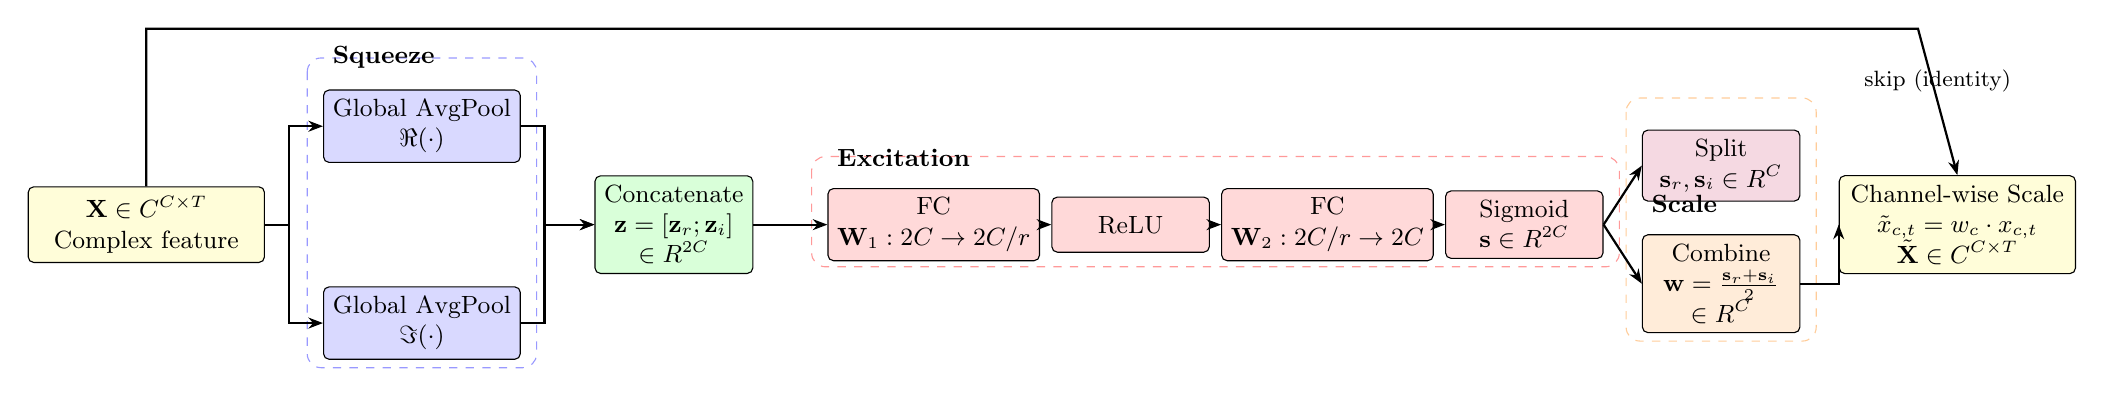
\begin{tikzpicture}[
    block/.style={rectangle, draw=black, fill=#1, minimum width=2.0cm, minimum height=0.7cm, align=center, font=\small, rounded corners=2pt},
    smallblock/.style={rectangle, draw=black, fill=#1, minimum width=1.8cm, minimum height=0.6cm, align=center, font=\footnotesize, rounded corners=2pt},
    arrow/.style={-{Stealth[scale=0.8]}, thick},
    % Color scheme
]

% ===== SQUEEZE =====
\node[block=blue!15] (squeeze_real) at (0, 2.5) {Global AvgPool\\$\Re(\cdot)$};
\node[block=blue!15] (squeeze_imag) at (0, 0.0) {Global AvgPool\\$\Im(\cdot)$};

% Input
\node[block=yellow!15, minimum width=3cm] (input) at (-3.5, 1.25) {$\mathbf{X} \in \mathbb{C}^{C \times T}$\\Complex feature};
\draw[arrow] (input.east) -- ++(0.3,0) |- (squeeze_real.west);
\draw[arrow] (input.east) -- ++(0.3,0) |- (squeeze_imag.west);

% ===== CONCAT =====
\node[block=green!15] (concat) at (3.2, 1.25) {Concatenate\\$\mathbf{z} = [\mathbf{z}_r; \mathbf{z}_i]$\\$\in \mathbb{R}^{2C}$};
\draw[arrow] (squeeze_real.east) -- ++(0.3,0) |- (concat.west);
\draw[arrow] (squeeze_imag.east) -- ++(0.3,0) |- (concat.west);

% ===== EXCITATION =====
\node[block=red!15] (fc1) at (6.5, 1.25) {FC\\$\mathbf{W}_1: 2C \to 2C/r$};
\node[block=red!15] (relu) at (9.0, 1.25) {ReLU};
\node[block=red!15] (fc2) at (11.5, 1.25) {FC\\$\mathbf{W}_2: 2C/r \to 2C$};
\node[block=red!15] (sigmoid) at (14.0, 1.25) {Sigmoid\\$\mathbf{s} \in \mathbb{R}^{2C}$};
\draw[arrow] (concat.east) -- (fc1.west);
\draw[arrow] (fc1.east) -- (relu.west);
\draw[arrow] (relu.east) -- (fc2.west);
\draw[arrow] (fc2.east) -- (sigmoid.west);

% ===== SPLIT + SCALE =====
\node[block=purple!15] (split) at (16.5, 2.0) {Split\\$\mathbf{s}_r, \mathbf{s}_i \in \mathbb{R}^{C}$};
\node[block=orange!15] (weight) at (16.5, 0.5) {Combine\\$\mathbf{w} = \frac{\mathbf{s}_r + \mathbf{s}_i}{2}$\\$\in \mathbb{R}^{C}$};
\draw[arrow] (sigmoid.east) -- (split.west);
\draw[arrow] (sigmoid.east) -- (weight.west);

% ===== SCALE OUTPUT =====
\node[block=yellow!15, minimum width=3cm] (output) at (19.5, 1.25) {Channel-wise Scale\\$\tilde{x}_{c,t} = w_c \cdot x_{c,t}$\\$\tilde{\mathbf{X}} \in \mathbb{C}^{C \times T}$};
\draw[arrow] (weight.east) -| (output.west);
\draw[arrow] (input.north) -- ++(0, 2.0) -- ++(19.5+3, 0) -- (output.north) node[midway, above, font=\footnotesize] {skip (identity)};

% Labels
\node[font=\small\bfseries, above=0.15cm of squeeze_real.north west, anchor=south west] {Squeeze};
\node[font=\small\bfseries, above=0.15cm of fc1.north west, anchor=south west] {Excitation};
\node[font=\small\bfseries, above=0.15cm of weight.north west, anchor=south west] {Scale};

% Background boxes
\begin{scope}[on background layer]
\draw[blue!40, dashed, rounded corners=5pt]
    ($(squeeze_real.north west)+(-0.2,0.4)$) rectangle ($(squeeze_imag.south east)+(0.2,-0.1)$);
\draw[red!40, dashed, rounded corners=5pt]
    ($(fc1.north west)+(-0.2,0.4)$) rectangle ($(sigmoid.south east)+(0.2,-0.1)$);
\draw[orange!40, dashed, rounded corners=5pt]
    ($(split.north west)+(-0.2,0.4)$) rectangle ($(weight.south east)+(0.2,-0.1)$);
\end{scope}

\end{tikzpicture}
\end{document}
